\subsection{Reference model}
\label{sec:result_VCT_regression}
Before assessing the physical correctness of the ID regression models, the physical correctness of the Reference model must first be assessed. Standard manoeuvring model tests are used for this purpose. As a first step, total forces and moments from the model test are estimates with inverse dynamics (see \autoref{sec:inverse_dynamics}). These forces can be compared with corresponding forces predicted with the Reference model. 
\autoref{fig:VCT_regression_ID} shows such a comparison for a zigzag20/20 model test. The first graph shows the rudder signal $\delta$ together with drift angle $\beta$ and yaw rate $r$. A comparison of sway force $Y_D$ and yawing moment $N_D$ are shown in the other two graphs. The forces and moments predicted with the Reference model are in reasonable agreement with the forces from the experiment. There are small deviations, where the Reference model over predicts the forces and moments in the peaks -- in the ends of the counter rudder excitations. The predicted force signals seem to have the same general shape as the experimental forces, which implies that the Reference model captures most of the essential physics involved in the experiment and is therefore a relevant reference, when the physical correctness of the ID regressions should be assessed. 
\begin{figure}[h!]
    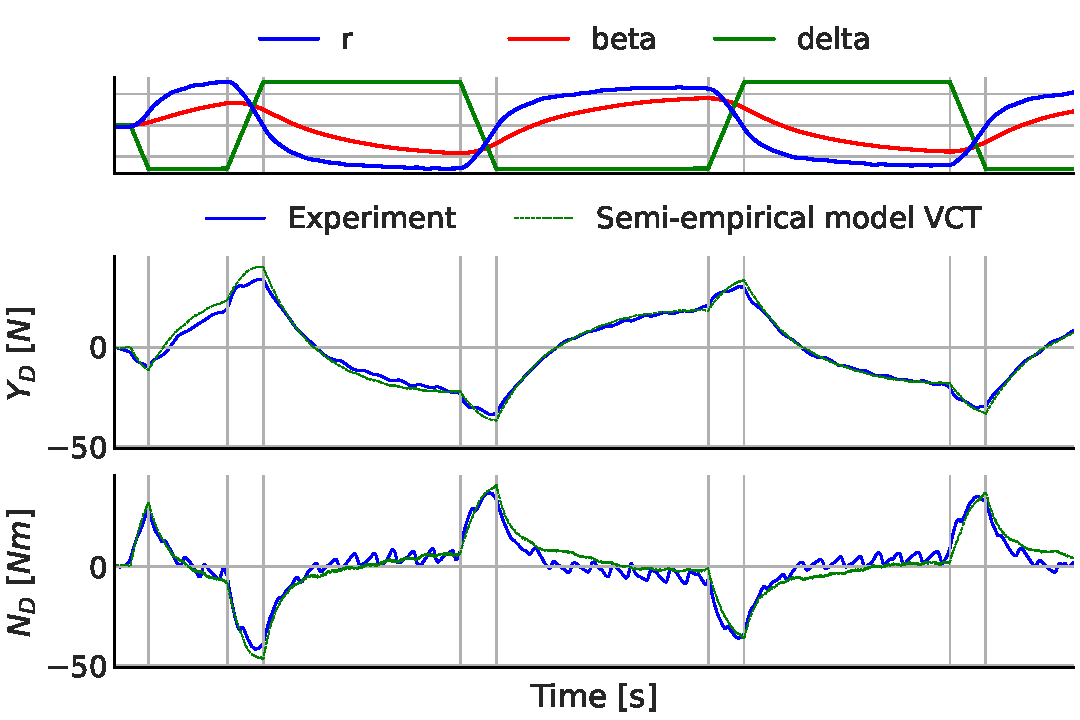
\includegraphics[width=\columnwidth]{figures/result_VCT_regression.VCT_regression_ID.pdf}
    \caption{Comparison of the total forces acting on the ship: predicted with the Semi-empirical VCT model, and the corresponding values from a zigzag20/20 test estimated with inverse dynamics.}
    \label{fig:VCT_regression_ID}
\end{figure}

\begin{table}[h!]
    \centering
    \caption{}
    \label{tab:vct_variations}
    \pgfplotstabletypeset[col sep=comma,fixed,precision=0,
    %columns={Test type,$u$,$v$,$r$,$\delta$,$\eta_0$},
    columns/Description/.style={string type, column type=l},
    columns/$V$/.style={fixed,precision=2},
    %columns/$u$/.style={string type},
    %columns/$v$/.style={string type},
    %columns/$r$/.style={string type},
    %columns/delta/.style={string type},
    %columns/$eta_0$/.style={string type},
    %columns/SI unit/.style={string type},
    %columns/Physical quantity/.style={string type},
    %columns/Denominator/.style={string type},
    %column type=l,	% specify the align method
    %every head row/.style={before row=\hline,after row=\hline},	% style the first row
    %every last row/.style={after row=\hline},	% style the last row
    ]{"tables/result_VCT_regression.reference_model_mean_average_error.csv"}
\end{table}